\documentclass[tikz,border=5pt]{standalone}
\usepackage{amsmath,amssymb}
\usetikzlibrary{angles,quotes}

\begin{document}
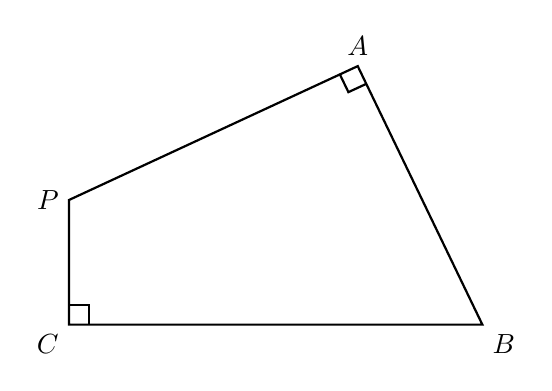
\begin{tikzpicture}[thick, scale=1]
  % 顶点坐标
  \coordinate (C) at (0,0);
  \coordinate (B) at (5.25,0);
  \coordinate (A) at (3.667,3.283);
  \coordinate (P) at (0,1.583);

  % 四边形边线（原 D 点改为 P，位置与连线保持不变）
  \draw (P) -- (A) -- (B) -- (C) -- cycle;

  % 直角标记
  \draw pic[draw, angle radius=0.25cm] {right angle=P--A--B};
  \draw pic[draw, angle radius=0.25cm] {right angle=P--C--B};

  % 顶点标签
  \node[above] at (A) {$A$};
  \node[below right] at (B) {$B$};
  \node[below left] at (C) {$C$};
  \node[left] at (P) {$P$};
\end{tikzpicture}
\end{document}
